\section{Prototype Car}

\begin{figure}[ht!]
    \centering
    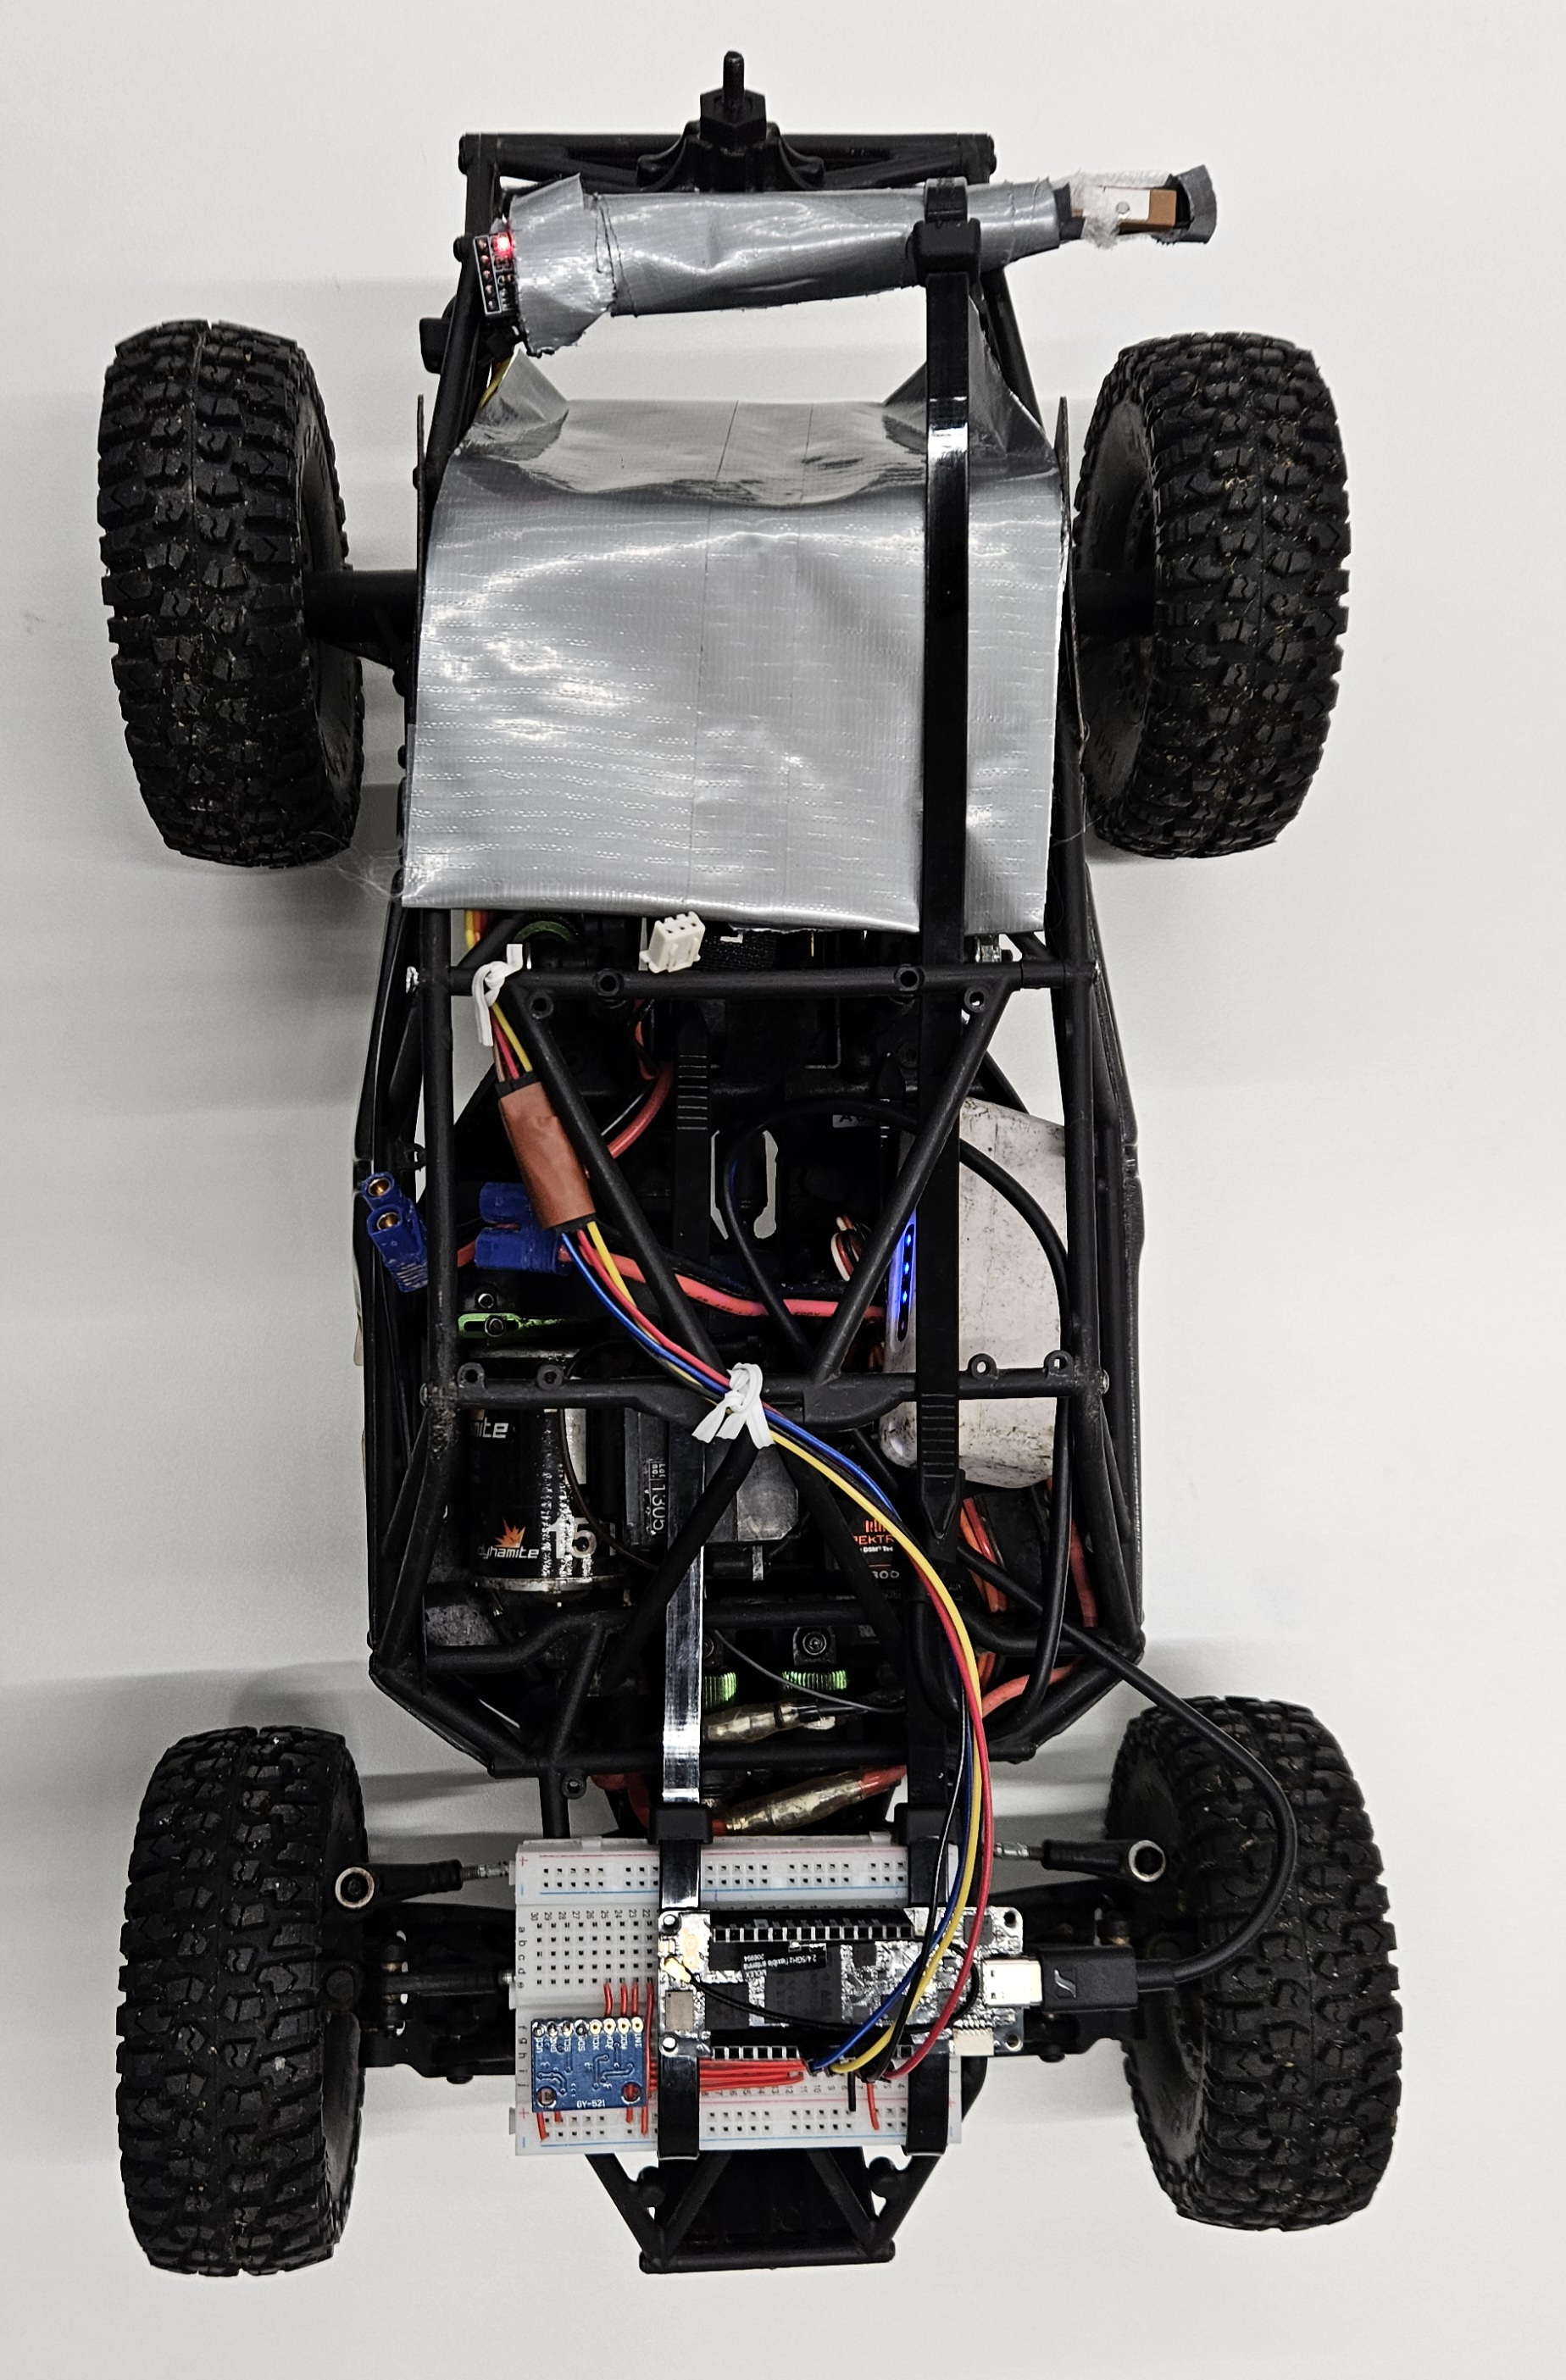
\includegraphics[angle=90,width=0.7\textwidth]{../../assets/images/roadsense_rc_top.jpg}
    \caption{RoadSense Prototype RC Top View}
\end{figure}

\subsubsection{Hardware Components}

\begin{enumerate}
    \item \textbf{Microcontroller}: \\
        \textbf{Arduino Portenta H7} with built-in Wi-Fi capability and RTOS support. \\
        Enables usage of threads for sensor data collection and transmission.
    \item \textbf{IMU Sensor}: \\
        \textbf{GY-521} with MPU6050 6DOF (3-Axis Gyro and 3-Axis Accelerometer). \\
        While currently only the z-axis acceleration is used, the sensor provides additional data which can be used for future work to improve the road state qualification model.
    \item \textbf{GPS Module}: \\
        \textbf{DFRobot GPS + BDS BeiDou} with output of position and speed. \\
        We were able to fix connectivity by integrating EMF shielding. As the transmitted speed data was faulty, we had to make use of a fallback solution by approximating each segment through a fixed time of 3 seconds.
    \item \textbf{EMF Shielding}: \\
        \textbf{DIY} using aluminum foil to shield the GPS module from electromagnetic interference.

\end{enumerate}

Detailed information on the pin connections for the sensors with the Arduino Portenta H7 can be found in Table \ref{tab:sensor_connections}.

\begin{table}[h!]
    \centering
    \begin{tabular}{|l|l|l|p{8cm}|}
    \hline
    \textbf{}         & \textbf{Sensor}       & \textbf{Portenta H7}            & \textbf{Description}                                                    \\ \hline
    \textbf{GY-521}         & VCC                   & 3.3V                            & Power supply (3.3V)                                                     \\ \cline{2-4}
                            & GND                   & GND                             & Ground                                                                  \\ \cline{2-4}
                            & SDA                   & SDA (Pin 11)                    & I2C Data line (SDA)                                                     \\ \cline{2-4}
                            & SCL                   & SCL (Pin 12)                    & I2C Clock line (SCL)                                                    \\ \hline
    \textbf{DFRobot GPS}    & VCC                   & 3.3V                            & Power supply (3.3V)                                                     \\ \cline{2-4}
                            & GND                   & GND                             & Ground                                                                  \\ \cline{2-4}
                            & TX                    & RX (Pin 13)                     & Serial data transmit line \newline (TX from GPS to RX on Portenta H7)   \\ \cline{2-4}
                            & RX                    & TX (Pin 14)                     & Serial data receive line \newline (RX from GPS to TX on Portenta H7)    \\ \hline
    \end{tabular}
    \caption{Pin Connections for Sensors with Arduino Portenta H7}
    \label{tab:sensor_connections}
    \end{table}